%=============================================================================
%  Anchored Semantic Reduction: Locating and Policing the Bottleneck of
%  Reliable AI for Mathematics
%
%  Compiles with pdfLaTeX/XeLaTeX.  Tables and figures are generated by
%  experiments/run_experiment.py and \input from paper/tables and paper/figures,
%  so every number in this paper is reproducible from the accompanying code.
%=============================================================================
\documentclass[11pt]{article}

\usepackage[T1]{fontenc}
\usepackage[utf8]{inputenc}
\usepackage[margin=1in]{geometry}
\usepackage{amsmath,amssymb,amsthm}
\usepackage{booktabs}
\usepackage{graphicx}
\usepackage{pgfplots}
\pgfplotsset{compat=1.18}
\usepackage{array}
\usepackage[hidelinks]{hyperref}
\usepackage{natbib}
\bibliographystyle{plainnat}

% Semantic brackets: define locally so no extra package is required.
\providecommand{\llbracket}{[\![}
\providecommand{\rrbracket}{]\!]}
\newcommand{\sem}[1]{\llbracket #1 \rrbracket}

% -- pipeline names, spelled exactly as they appear in the generated tables ---
\newcommand{\pGen}{\textsf{gen\_only}}
\newcommand{\pVerify}{\textsf{verify}}
\newcommand{\pLex}{\textsf{verify+lexical\_anchors}}
\newcommand{\pTyp}{\textsf{verify+typed\_anchors}}
\newcommand{\pTypAnch}{\textsf{typed\_anchored}}
\newcommand{\pTypBest}{\textsf{typed\_best\_effort}}
\newcommand{\pOracle}{\textsf{oracle}}
\newcommand{\Alex}{\textsf{A-lex}}
\newcommand{\Atype}{\textsf{A-type}}

\newtheorem{theorem}{Theorem}
\newtheorem{proposition}{Proposition}
\newtheorem{corollary}{Corollary}
\theoremstyle{definition}
\newtheorem{definition}{Definition}
\newtheorem{remark}{Remark}

\title{\bfseries Anchored Semantic Reduction:\\ Locating and Policing the Bottleneck of Reliable AI for Mathematics}

\author{%
  \textit{Author}\thanks{%
    Author block intentionally left generic. Replace before submission.
    The experimental code, the generated tables and figures, the AI
    collaboration log and the after-action review accompany this paper.}%
}

\date{\today}

\begin{document}
\maketitle

\begin{abstract}
\noindent
AI systems now produce mathematical arguments that are fluent, plausible, and
wrong. The dominant response is to add \emph{verification}: search-and-check
loops, formal proof assistants, and reproducible evaluation. We argue that this
response is aimed one layer too late. Decomposing an AI-for-mathematics (AI4Math)
pipeline into \emph{generation}, \emph{semantic reduction}, and
\emph{verification}, we show that the reliability of the whole pipeline is
normally governed by the middle layer --- the translation from natural language
into the object the verifier actually consumes --- and that this layer is
routinely left unmonitored. We give two propositions. The first is an
\emph{existence} result: because a sound-and-complete verifier can only be sound
\emph{relative to the object it is handed}, an unfaithful reduction yields a
certified, machine-checked, wrong answer. The second is a \emph{structural}
impossibility: any verifier that sees only the reduced object is a function of
that object, so it cannot separate two sentences the reduction conflates --- its
detection recall on such pairs is zero, not merely low.
We then build an exactly decidable experimental harness over a small typed
intermediate representation of finite-domain affine arithmetic, generate a
controlled corpus of semantics-changing perturbations across five failure
classes, and compare two ways of \emph{anchoring} the reduction: comparing
against a re-rendering of the intermediate object (\Alex), and asserting
independently extracted statements about meaning as predicates over that object
(\Atype). On a prevalence-controlled corpus, plain verification reports a
$55.9\%$ silent error rate while certifying $100\%$ of its answers; typed anchors
drive silent error to $0\%$. A further ablation at the canonical surface form
shows that \Alex's headline detection recall is partly a paraphrase artefact ---
it collapses to $0\%$ on typing drift --- whereas \Atype{} reaches $100\%$ recall
with no certification cost. We close with an eight-item reliability checklist and
an explicit statement of the conditions under which anchoring cannot help.
\end{abstract}

\section{Introduction}
\label{sec:intro}

An AI system asked to settle a mathematical question will, today, usually give an
answer that reads as if it had been reasoned out. Sometimes it has been. The
problem that has organised the field is that the two cases are hard to tell
apart: a model can produce a derivation whose every step looks locally
reasonable, which reaches a conclusion that is false, and which no one catches
because the derivation is only ever read, never checked
\citep{yang2024formalreasoning}. The failures are not noise. They are
systematic, they survive scale, and they are most likely precisely where the
problem is hard.

The community's main answer has been \emph{verification}. Three strands are
visible. The first pairs a generative model with a search-and-check loop, so
that candidate steps are evaluated before being extended
\citep{lightman2024verify,uesato2022processoutcome}. The second replaces
natural-language argument with formal proof, so that a machine checks every
inference and a proof cannot be subtly wrong
\citep{demoura2021lean4,hubert2025alphaproof,trinh2024alphageometry}; the
translation step that carries a problem from prose into the formal system is
autoformalization \citep{wu2022autoformalization,jjiang2023draftsketchprove}.
The third makes evaluation reproducible and comparable across systems
\citep{zheng2022minif2f,romeraparedes2024funsearch,charton2024patternboost}.
Each strand has produced genuine, durable progress.

This paper makes a claim about \emph{where} that progress has to be applied, and
about what happens when it is applied everywhere except there. Consider a
pipeline in the abstract:
\[
  \underbrace{\text{statement}}_{\text{natural language}}
  \;\longrightarrow\;
  \underbrace{\text{object}}_{\text{what the checker eats}}
  \;\longrightarrow\;
  \underbrace{\text{verdict}, \text{certificate}}_{\text{checked}}
\]
The middle arrow is a \emph{semantic reduction}. It is where the meaning of an
informal sentence is fixed. It is also, in most systems, a preprocessing
detail: the model's reading of the problem is passed straight to the checker, and
the checker is trusted because it is sound. We argue that this is a category
error. A checker is sound \emph{relative to the object it is handed}. If the
object is not what the sentence meant, soundness buys nothing at all, and the
resulting answer is not merely unverified --- it is verified and wrong, which is
strictly worse than an answer that was obviously a guess.

The contribution of this paper is to make that argument precise, then to test it.

\paragraph{Contributions.}
\begin{enumerate}
  \item \textbf{A three-layer error model} (\S\ref{sec:framework}) that separates
        generation, semantic reduction, and verification, and localises
        reliability in the middle layer. We argue that most reported AI4Math
        reliability failures are reduction failures wearing a verification
        costume.
  \item \textbf{A failure taxonomy of the reduction layer}
        (\S\ref{sec:taxonomy}): quantifier drift, domain-kind (typing) drift,
        strictness drift, assumption omission, and vacuity. The taxonomy is
        instantiated and measured, not merely proposed.
  \item \textbf{Two propositions} (\S\ref{sec:props}). Proposition~\ref{prop:sound}
        shows that certified wrongness is reachable even when the verifier is
        exactly sound and complete. Proposition~\ref{prop:blind} shows that an
        IR-only verifier has detection recall \emph{identically zero} on pairs
        the reduction collapses --- a structural statement, not an empirical
        accident.
  \item \textbf{An exactly decidable experimental harness}
        (\S\ref{sec:setup}). The intermediate representation is a typed,
        finite-domain affine fragment decided by exact enumeration over rationals,
        so no floating-point tolerance can mask an error, and the whole study is
        deterministic given a seed.
  \item \textbf{A comparative result on anchoring}
        (\S\ref{sec:results}). Lexical round-trip anchors (\Alex) and typed
        predicated anchors (\Atype) are measured as reduction-error detectors.
        We show which of them is honest and why, including an ablation at the
        canonical surface form that removes a paraphrase confound from \Alex.
  \item \textbf{An eight-item reliability checklist} (\S\ref{sec:checklist}) and
        a statement of the conditions under which anchoring \emph{cannot} help
        (\S\ref{sec:limits}).
\end{enumerate}

We are explicit about what we do \emph{not} claim. We do not claim that formal
verification is unnecessary; we claim it is insufficient on its own. We do not
claim that our controlled language is natural language; it is a deliberately
small, fully specified fragment whose semantics are exact, which is what makes
the measurements trustworthy. And we do not claim that anchors work
unconditionally: \S\ref{sec:limits} states the independence condition they
require, and what happens when it fails.

\section{Related Work}
\label{sec:related}

\paragraph{Step-level supervision and verification of informal reasoning.}
\citet{uesato2022processoutcome} ran the first systematic comparison of
outcome-based against process-based supervision on a natural-language reasoning
task, finding that outcome-only supervision reaches similar final-answer accuracy
with fewer labels while failing to reduce reasoning errors among correct answers.
\citet{lightman2024verify} scaled the process-supervised reward model to the MATH
dataset with 800{,}000 step-level human labels and showed a clear advantage for
process supervision under best-of-$N$ reranking ($78.2\%$ against $72.4\%$ for
an outcome-supervised model). This line of work is, in our terms, about
\emph{which step to believe}. It improves the generation layer and adds a
checking signal over steps. It does not, however, monitor whether the problem was
read correctly in the first place --- a process reward model scores a *given*
chain of reasoning, and a uniformly well-scored chain restating the wrong
question is still wrong.

\paragraph{Formal proof and autoformalization.}
Formal systems remove the bottom of the error stack: a proof that type-checks
cannot be subtly invalid \citep{demoura2021lean4}. This has been turned into
systems that reach olympiad-level performance within the formal environment
\citep{trinh2024alphageometry,hubert2025alphaproof}. But the formal environment
must be entered. Autoformalization is the bridge: \citet{wu2022autoformalization}
showed that large language models translate a substantial fraction of competition
problems correctly into Isabelle/HOL --- and, importantly, reported that a
significant fraction is \emph{not} translated correctly, with the failures being
of exactly the character our taxonomy describes. \citet{jiang2023draftsketchprove}
route informal proofs through formal sketches to guide a prover, raising the
solve rate from $20.9\%$ to $39.3\%$, again with the informal-to-formal mapping as
the critical, and lightly supervised, component.

Our contribution relative to this literature is not a better translator. It is a
statement about what a translator must be paired with in order for the pipeline
to be trustworthy at all, together with an empirical demonstration that the
obvious pairing --- the round-trip --- is not it.

\paragraph{Program search, constructions and counterexamples.}
\citet{romeraparedes2024funsearch} pair a language model with a systematic
evaluator and search in program space, obtaining new constructions for the cap
set problem; \citet{charton2024patternboost} alternate local search with a
transformer to find extremal constructions, including a counterexample to a
conjecture open for thirty years. These systems are protected by an evaluator
that is exact for the object being searched. They are the positive control for
our argument: reliability comes from having \emph{some} layer whose semantics are
fixed and checkable, and from keeping the generative layer away from it.

\paragraph{Surveys and positioning.}
\citet{yang2024formalreasoning} argue that formal mathematical reasoning is the
avenue most likely to carry AI4Math beyond its current ceiling, and identify
autoformalization as a central open problem. Our paper takes that assessment
seriously and sharpens it: the open problem is not only \emph{how to translate
better}, but \emph{how to know when a translation is wrong}, which is a
monitoring problem rather than a modelling problem, and admits a structural
impossibility result.

\section{Framework: Anchored Semantic Reduction}
\label{sec:framework}

\subsection{Three layers, and where the errors enter}

We decompose an AI4Math pipeline into three layers.

\begin{definition}[Three-layer pipeline]
\label{def:layers}
A pipeline consists of
\begin{enumerate}
  \item a \emph{generation} map $G$ that produces a natural-language answer,
        argument, or question from a problem statement $s$;
  \item a \emph{semantic reduction} $R$ that maps a natural-language statement to
        an intermediate representation (IR) $S = R(s)$;
  \item a \emph{verification} map $V$ that maps an IR to a verdict and, ideally, a
        machine-checkable certificate.
\end{enumerate}
The pipeline's \emph{answer} on $s$ is $V(R(s))$. Write $\llbracket S
\rrbracket$ for the truth value the IR $S$ denotes, and $\rho^\ast$ for the
\emph{faithful} reduction, i.e.\ the one satisfying $\llbracket \rho^\ast(s)
\rrbracket = \mathrm{truth}(s)$ for every sentence $s$ in the domain of interest.
Then $R$ is \emph{faithful on} $s$ iff $R(s) = \rho^\ast(s)$, and \emph{unfaithful
on} $s$ otherwise.
\end{definition}

Note the asymmetry in Definition~\ref{def:layers}. Faithfulness is a property of
$R$; soundness is a property of $V$. The literature's investment is concentrated
in $V$. The next subsection shows why that is not enough.

\subsection{A typed IR over a decidable fragment}
\label{sec:ir}

For the experiment we need an IR whose semantics are exact and whose verdicts are
reproducible to the bit. We use a small typed fragment.

\begin{definition}[IR]
\label{def:ir}
A specification $S$ is a tuple $(\mathcal{V}, H, g, Q)$ where
\begin{itemize}
  \item $\mathcal{V} = \{(v_i, \ell_i, u_i)\}$ declares each variable $v_i$ as an
        integer constrained to a finite closed interval $[\ell_i, u_i]$;
  \item $H = \{h_1, \dots, h_p\}$ is a finite set of hypotheses, each a linear
        constraint $\sum_j c_j v_j \bowtie k$ with rational coefficients $c_j$,
        rational $k$, and $\bowtie \;\in \{<, \le, =, \ge, >\}$;
  \item $g$ is a goal, of the same form;
  \item $Q \in \{\mathsf{EXISTS}, \mathsf{FORALL}\}$ is the \emph{quantifier of the
        question}: is $g$ satisfiable together with $H$, or does $H$ entail $g$?
\end{itemize}
\end{definition}

The quantifier is part of the IR deliberately: dropping it is one of the failure
modes we study. Decisions are computed by exact enumeration of the declared box
using rational arithmetic (\texttt{fractions.Fraction} in Python), so a verdict,
and the ground truth it is compared against, are exact integers or exact
rationals throughout --- there is no tolerance to tune and none to hide behind.
The fragment is decidable and the procedure is sound \emph{and} complete inside
it, which is the point: we want a verifier that cannot be blamed.

\subsection{Failure taxonomy of the reduction layer}
\label{sec:taxonomy}

The following five classes are the reduction errors our corpus instantiates.
Each is a distinct way for two sentences with different truth values to
collapse, or for a claim to become true for the wrong reason.

\begin{definition}[Reduction failure classes]
\label{def:taxonomy}
Let $s$ be a statement and $R(s)$ its IR.
\begin{description}
  \item[P1 Quantifier drift.] $s$ asks a universal question; $R(s)$ encodes an
        existential one (or conversely). ``For every $x$'' becomes ``for some
        $x$''.
  \item[P2 Domain-kind (typing) drift.] $s$ restricts the domain \emph{by kind}
        (``positive'', ``non-negative'', ``arbitrary''); $R(s)$ records only an
        interval and loses the kind, so a boundary witness the sentence excluded
        becomes admissible.
  \item[P3 Strictness drift.] $s$ uses a strict inequality; $R(s)$ weakens it
        (or conversely), which changes the answer exactly at the extreme the
        comparison pins down.
  \item[P4 Assumption omission.] $s$ carries a qualifying clause (``and $x$ is a
        multiple of $m$''); $R(s)$ drops it, so a hypothesis that removes the only
        witness disappears.
  \item[P5 Vacuity.] $s$ is a universal claim whose hypotheses admit no model in
        the declared box. It is therefore \emph{true}, but true of nothing; a
        pipeline that reports ``true'' without the warning has answered a
        different question from the one asked.
\end{description}
\end{definition}

P1--P4 are semantics-changing: the truth value flips. P5 is subtler --- the truth
value does not flip, but the \emph{informativeness} does, and P5 is the class most
likely to survive every accuracy-based check.

\subsection{Two propositions}
\label{sec:props}

\begin{proposition}[Certified wrongness]
\label{prop:sound}
Let $V$ be sound and complete for the IR fragment, so that $V(S) =
\llbracket S \rrbracket$ for every well-formed $S$. If $R$ is unfaithful on $s$
\emph{and} $\llbracket R(s) \rrbracket \neq \mathrm{truth}(s)$, then the pipeline
emits a verdict that carries a machine-checkable certificate and is wrong.
\end{proposition}

\begin{proof}
The pipeline answers $V(R(s))$. Faithfulness of $V$ gives $V(R(s)) = \llbracket
R(s) \rrbracket$. By hypothesis $\llbracket R(s) \rrbracket \neq
\mathrm{truth}(s)$, hence the emitted verdict differs from the truth. The
verdict remains accompanied by $V$'s certificate, which is internally valid: it
witnesses the verdict for the \emph{wrong} object. \qed
\end{proof}

Proposition~\ref{prop:sound} is why the combination of high accuracy and high
certificate rate is not reassuring on its own, and why we report silent error
rate --- wrong answers \emph{emitted as certified} --- separately from accuracy.
The proof is one line; the consequence is not obvious in practice, because a
pipeline that certifies everything looks like a pipeline that has been checked.

\begin{proposition}[Structural blind spot of IR-only verification]
\label{prop:blind}
Let $V$ be any verifier whose input is the IR alone, so $V$ is a function of $S$.
Let $s, s'$ be two statements with $R(s) = R(s')$ but $\mathrm{truth}(s) \neq
\mathrm{truth}(s')$. Then
\begin{enumerate}
  \item the verdicts agree, $V(R(s)) = V(R(s'))$, and so do the certificates;
  \item $V$ is wrong on at least one of $s, s'$;
  \item consequently, on the pair $(s, s')$, $V$'s detection recall is $0$.
\end{enumerate}
\end{proposition}

\begin{proof}
(1) Since $V$ is a function and $R(s) = R(s')$, we have $V(R(s)) = V(R(s'))$;
the certificate is part of $V$'s output, so it coincides too. (2) A single
verdict cannot equal two different truth values, so it differs from
$\mathrm{truth}(\cdot)$ on at least one member. (3) Detection requires the
verifier to signal a difference between the two cases; by (1) its output is
identical, so it signals nothing. \qed
\end{proof}

\begin{corollary}
\label{cor:stronger}
Replacing $V$ by a stronger or smarter IR-only verifier cannot raise recall above
$0$ on the class of pairs collapsed by $R$. Detection of reduction error is
therefore not obtainable by improving the verifier; it requires a source of
information that does not pass through $R$.
\end{corollary}

Corollary~\ref{cor:stronger} is the design constraint that motivates anchors. The
zero row in Table~\ref{tab:detectors} for ``IR verification alone'' is a
consequence of Proposition~\ref{prop:blind}, and we verify empirically that
$100\%$ of our critical pairs are collapsed in exactly this way
(\S\ref{sec:blindspot}).

\subsection{Anchors: lexical round-trip versus typed predicates}
\label{sec:anchors}

An \emph{anchor} is a statement about what a problem means, extracted from the
sentence by a route that does not pass through $R$. Anchors are what
Corollary~\ref{cor:stronger} demands. We compare two ways of turning an anchor
into a check.

\begin{definition}[\Alex, lexical round-trip]
\label{def:alex}
Render $R(s)$ back to a sentence $\hat{s}$ using a partial inverse of the
reductor, then compare $s$ and $\hat{s}$ slot by slot, by exact surface
equality. Report a violation when a slot differs. \emph{Semantically irrelevant}
differences --- synonyms --- are indistinguishable from relevant ones.
\end{definition}

\begin{definition}[\Atype, typed predicated anchors]
\label{def:atype}
Extract the anchors from $s$ with a separately declared grammar, then assert them
as \emph{predicates} over $R(s)$: the quantifier field, the declared domain as a
set, the \emph{solution set} of the goal over that domain, and the presence and
modulus of a congruence witness. Report a violation when a predicate is
contradicted.
\end{definition}

The difference is not cosmetic, and it is sharpest on P2. The IR has no slot for
domain \emph{kind}: it records only the resulting interval. A round-trip
therefore reproduces the interval faithfully and annihilates the type
information, so \Alex{} cannot see typing drift at all. \Atype{} can, because it
carries the intended typing rule on the anchor side: from ``positive'' it
computes the expected domain $\max(\ell, 1)$ and compares \emph{that} against the
IR's declared domain. The string route loses the type; the predicate route does
not.

\begin{remark}[Type erasure is invisible to round-tripping]
\label{rem:erasure}
Whenever a reduction is a non-injective quotient --- it forgets a distinction that
the surface language makes --- a round-trip check that compares against the
quotient's own rendering is structurally blind to exactly the forgotten
distinction. This is the general form of \Alex's P2 failure, and it means the
round-trip's blind spot is determined by the IR's \emph{expressive gaps}, not by
its accuracy.
\end{remark}

\subsection{A reliability checklist}
\label{sec:checklist}

The framework yields an operational checklist. It is short on purpose: every item
is a question with a yes/no answer, and a ``no'' is a specific, actionable defect.

\begin{enumerate}
  \item[\textbf{C1}] Is there an explicit intermediate object at all, or does the
        model's prose answer go straight to a human?
  \item[\textbf{C2}] Is the verifier's domain of competence stated --- which
        fragment, which logic, decidable or not?
  \item[\textbf{C3}] Is the reduction \emph{monitored}, or only the final answer?
  \item[\textbf{C4}] Does at least one check compare against the \emph{source
        statement}, rather than against a re-rendering of the intermediate
        object? (A ``no'' here means the pipeline is exposed to
        Remark~\ref{rem:erasure}.)
  \item[\textbf{C5}] Are unreadable or unconfirmed anchors treated as failures
        (abstain) or as passes (best effort), and is the chosen policy stated?
  \item[\textbf{C6}] Is vacuity distinguished from truth in the output?
  \item[\textbf{C7}] Are coverage, certification rate, and accuracy reported
        \emph{separately}? A pipeline can be accurate, certifying, and useless.
  \item[\textbf{C8}] Is the reduction failure taxonomy instantiated with held-out
        examples, as in \S\ref{sec:taxonomy}, and tested?
\end{enumerate}

\section{Experimental Design}
\label{sec:setup}

\subsection{Controlled language and corpus}
\label{sec:corpus}

We work in a controlled natural language whose semantic content is a record of
four feature families: \emph{quantifier}, \emph{adjective} (the domain kind),
\emph{strictness} (the comparison), and \emph{qualifier} (an optional congruence
clause). Each family admits several synonymous surface realisations, so the same
meaning can be written in many ways. The reductor translates a feature record to
the IR of Definition~\ref{def:ir} and may be \emph{blind} to any subset of the
families --- a blind reductor silently normalises away a distinction it does not
model, exactly as a language model does when it paraphrases a problem into its
own reading.

Two modelling decisions make the measurements interpretable, and we state them
because conflating them is the easiest way to produce a misleading result.

\paragraph{The reductor and the anchor extractor have different defects.}
The reductor is given \emph{full} linguistic competence (it reads every synonym)
but is blind to all four feature families: its defect is semantic, not lexical.
The anchor extractor is a symbolic component with a \emph{declared, closed}
grammar: its defect is coverage, not semantics. Keeping these separate means a
lexicon gap and a semantic blindness cannot be confused in the tables.

\paragraph{The corpus is split so that detection and cost are measurable.}
The \emph{critical} set contains base--perturbed pairs, one pair per perturbation
in each class, admitted only after checking that the ground truth actually
flips; a perturbation that does not flip the truth value is discarded at
generation time. The \emph{benign} set contains strictly meaning-preserving
paraphrases drawn from a population on which the blind reductor is provably
faithful; here no answer is wrong, so every abstention is a pure certification
cost. Without this split, a reductor blind to four families at once leaves almost
no faithful instances against which to measure the price. We also report a
\emph{prevalence-controlled} corpus (every base instance plus $20\%$ of the
perturbed ones) because the balanced critical set inflates absolute error rates
by construction.

\subsection{Pipelines}
\label{sec:pipelines}

We compare seven rungs, chosen so that each step changes exactly one thing. Their
names in the tables are given verbatim in parentheses.

\begin{itemize}
  \item \pGen{} --- layer 1 alone: the model's reading, no IR, no certificate.
  \item \pVerify{} --- reduce, then decide the IR exactly. Sound and complete
        \emph{on the IR}.
  \item \pLex{} --- blind reduction, then an \Alex{} check; abstain unless every
        anchor is readable and holds.
  \item \pTyp{} --- blind reduction, then an \Atype{} check; same conservative
        policy.
  \item \pTypAnch{} --- \emph{faithful} reduction, then an \Atype{} check;
        abstain unless certifiable.
  \item \pTypBest{} --- faithful reduction; answer always, certify only when the
        anchors confirm.
  \item \pOracle{} --- faithful reduction, perfect anchors: the ceiling.
\end{itemize}

The faithful reduction in the last three rungs is a \emph{target}, not a claim
that a real system attains it. Its role is to decompose the problem: the first
three rungs isolate what anchors buy under an unfaithful reduction, and the last
three isolate what is left once the reduction itself is trustworthy. A real
system approximates the latter by restricting the accepted input to a language it
can translate faithfully and abstaining outside it --- which is exactly how formal
and controlled-language front ends behave.

\subsection{Metrics}
\label{sec:metrics}

We report four quantities per pipeline. \emph{Coverage} is the fraction of
instances answered. \emph{Accuracy}$\,\mid\,$\emph{answered} conditions on having
answered. \emph{Silent error rate} is the fraction of \emph{all} instances on
which a wrong answer was emitted \emph{as if certified} --- the quantity that
Proposition~\ref{prop:sound} says can coexist with a perfect certificate rate.
\emph{Certificate rate} is the fraction carrying a machine-checkable object.

For the anchors themselves we report three quantities, because ``detected'' and
``refused to answer'' are not the same thing. An instance is \emph{unfaithful}
when the blind reductor's IR differs from the reference IR built from the
sentence's true features --- a property of the reduction, not of the answer.
\emph{Recall} counts violations: the anchor \emph{contradicts} the IR, which is
genuine detection. \emph{Safety} counts unfaithful reductions whose answer was
withheld for any reason. \emph{Over-abstention} is the price: the share of
faithful reductions refused certification.

\section{Results}
\label{sec:results}

\subsection{The blind spot is real}
\label{sec:blindspot}

Across all $192$ critical pairs, the blind reductor produced an IR \emph{identical}
for both members in $100\%$ of cases, and the verifier returned an
\emph{identical} verdict in $100\%$ of cases. This is Proposition~\ref{prop:blind}
observed rather than assumed: the two sentences differ in truth value, and the
entire pipeline, up to and including its certificate, cannot tell them apart.
Any claim to the contrary would have to come from information that never entered
the IR.

\subsection{What verification alone buys, and what anchors buy}
\label{sec:pipelinesresults}

\begin{figure}[t]
  \centering
  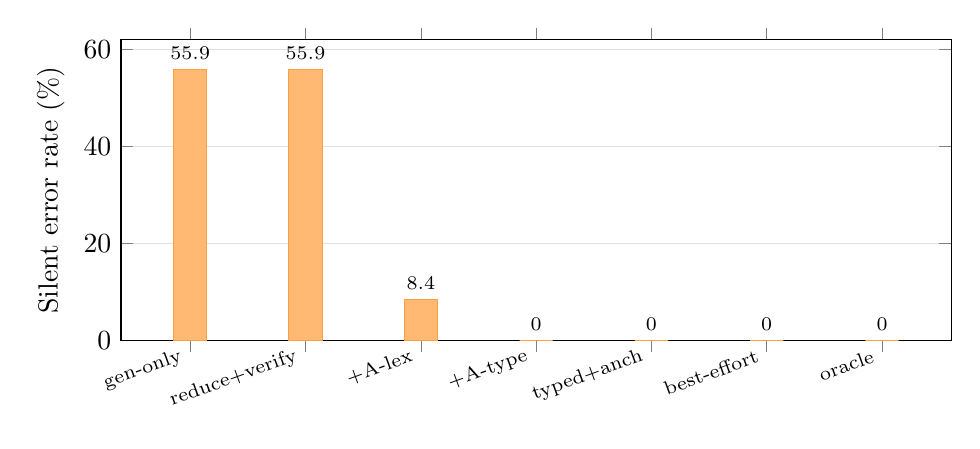
\begin{tikzpicture}
\begin{axis}[
  ybar, bar width=12pt, width=\linewidth, height=5.4cm,
  ylabel={Silent error rate (\%)}, ymin=0, ymax=62,
  symbolic x coords={gen-only,reduce+verify,+A-lex,+A-type,typed+anch,best-effort,oracle},
  xtick=data, x tick label style={rotate=20, anchor=east, font=\scriptsize},
  enlarge x limits=0.10, ymajorgrids, grid style={draw=black!12},
  nodes near coords, nodes near coords style={font=\scriptsize},
]
\addplot[fill=orange!55, draw=orange!75] coordinates {(gen-only,55.9) (reduce+verify,55.9) (+A-lex,8.4) (+A-type,0.0) (typed+anch,0.0) (best-effort,0.0) (oracle,0.0)};
\end{axis}
\end{tikzpicture}

  \caption{Silent error rate --- wrong answers emitted as certified --- on the
  prevalence-controlled corpus ($n = 238$). Reduction plus exact verification
  (\pVerify) is the worst of both worlds: it certifies every answer and inherits
  every reduction error. Adding anchors removes the certified wrongness; making
  the reduction faithful removes the error itself.}
  \label{fig:silent}
\end{figure}

\begin{table}[t]
\centering
\caption{Behaviour on semantics-changing tasks (base + perturbed members of every critical pair). Coverage is the fraction answered; silent error rate counts wrong answers that were emitted as if certified; certificate rate is the fraction carrying a machine-checkable object.}
\label{tab:critical}
\small
\begin{tabular}{lrrrrr}
\toprule
Pipeline & $n$ & Coverage & Acc.\,$\mid$\,ans. & Silent err. & Cert. rate \\
\midrule
gen\_only & 384 & 100.0 & 50.0 & 50.0 & 0.0 \\
verify & 384 & 100.0 & 50.0 & 50.0 & 100.0 \\
verify+lexical\_anchors & 384 & 26.6 & 80.4 & 5.2 & 26.6 \\
verify+typed\_anchors & 384 & 19.8 & 100.0 & 0.0 & 19.8 \\
typed\_anchored & 384 & 50.5 & 100.0 & 0.0 & 50.5 \\
typed\_best\_effort & 384 & 97.9 & 100.0 & 0.0 & 50.5 \\
oracle & 384 & 100.0 & 100.0 & 0.0 & 100.0 \\
\bottomrule
\end{tabular}
\end{table}


\begin{table}[t]
\centering
\caption{Behaviour on a prevalence-controlled corpus: every base instance plus $20\%$ of the perturbed ones. Unlike Table~\ref{tab:critical} this is not balanced, so the absolute silent error rates are the ones a deployment of this shape would face.}
\label{tab:mixed}
\small
\begin{tabular}{lrrrrr}
\toprule
Pipeline & $n$ & Coverage & Acc.\,$\mid$\,ans. & Silent err. & Cert. rate \\
\midrule
gen\_only & 238 & 100.0 & 44.1 & 55.9 & 0.0 \\
verify & 238 & 100.0 & 44.1 & 55.9 & 100.0 \\
verify+lexical\_anchors & 238 & 21.4 & 60.8 & 8.4 & 21.4 \\
verify+typed\_anchors & 238 & 11.8 & 100.0 & 0.0 & 11.8 \\
typed\_anchored & 238 & 48.7 & 100.0 & 0.0 & 48.7 \\
typed\_best\_effort & 238 & 96.6 & 100.0 & 0.0 & 48.7 \\
oracle & 238 & 100.0 & 100.0 & 0.0 & 100.0 \\
\bottomrule
\end{tabular}
\end{table}


Table~\ref{tab:critical} shows the balanced critical set, where half the
instances are by construction a semantics-changing edit; Table~\ref{tab:mixed} is
the headline. The second row is the one to look
at. \pVerify{} answers every question, is correct on $44.1\%$ of them, and
attaches a valid certificate to $100\%$ of its answers. Its silent error rate is
$55.9\%$: more than half of all queries receive a machine-checked wrong answer.
This is not a bug in the verifier --- the verifier is sound and complete. It is
Proposition~\ref{prop:sound} operating at scale.

The anchors move the certified wrongness. \pLex{} cuts silent error to $8.4\%$ and
\pTyp{} to $0\%$, at the cost of coverage: under the conservative
``abstain unless every anchor is readable and holds'' policy, the blind-reduction
rungs can only certify a fifth or a tenth of the corpus. That is the honest
trade: anchors do not make an unfaithful reduction correct, they make it
\emph{refuse to certify}. Reading the two levers together, the practical
operating points are \pTyp{}+ (\pTypAnch) for a conservative system that certifies
about half of what it sees with no silent error, and \pTypBest{} for a
best-effort system that answers almost everything ($96.6\%$ coverage) with no
silent error while honestly marking only $48.7\%$ as certified.

\begin{figure}[t]
  \centering
  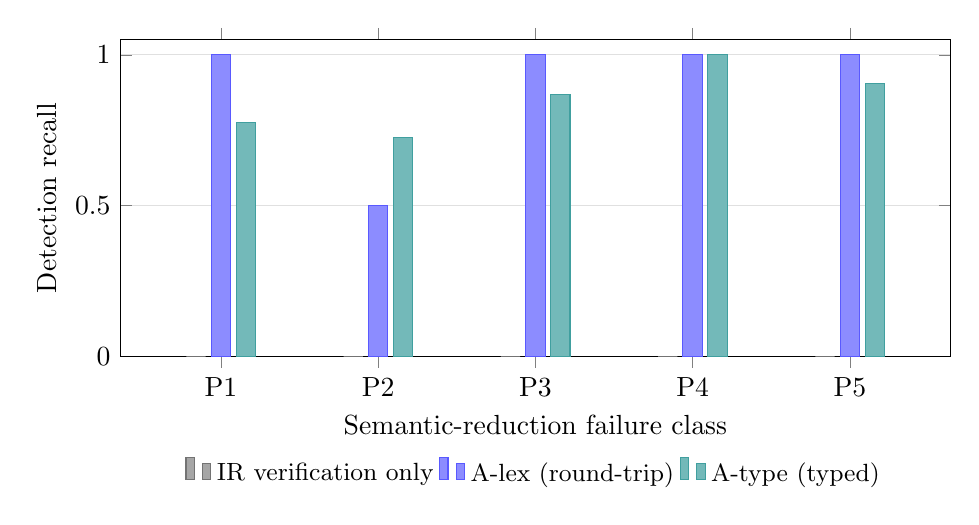
\begin{tikzpicture}
\begin{axis}[
  ybar, bar width=7pt, width=\linewidth, height=5.6cm,
  ylabel={Detection recall}, ymin=0, ymax=1.05,
  xlabel={Semantic-reduction failure class},
  symbolic x coords={P1,P2,P3,P4,P5}, xtick=data,
  enlarge x limits=0.16, ymajorgrids, grid style={draw=black!12},
  legend style={at={(0.5,-0.30)}, anchor=north, legend columns=3, font=\small, draw=none},
]
\addplot[fill=black!35, draw=black!55] coordinates {(P1,0.000) (P2,0.000) (P3,0.000) (P4,0.000) (P5,0.000)};
\addlegendentry{IR verification only}
\addplot[fill=blue!45, draw=blue!65] coordinates {(P1,1.000) (P2,0.500) (P3,1.000) (P4,1.000) (P5,1.000)};
\addlegendentry{A-lex (round-trip)}
\addplot[fill=teal!55, draw=teal!75] coordinates {(P1,0.775) (P2,0.725) (P3,0.867) (P4,1.000) (P5,0.906)};
\addlegendentry{A-type (typed)}
\end{axis}
\end{tikzpicture}

  \caption{Detection recall by failure class. IR verification alone is zero
  everywhere by Proposition~\ref{prop:blind}. \Alex{} is strong but non-monotone;
  \Atype{} trades a little recall for uniform safety. The $p{=}1.00$ ablation in
  Table~\ref{tab:canonical} shows that part of \Alex's apparent recall is
  paraphrase sensitivity rather than semantic detection.}
  \label{fig:recall}
\end{figure}

\subsection{Detection, safety, and the price of abstention}
\label{sec:detectors}

\begin{table}[t]
\centering
\caption{Mechanisms as detectors of \emph{unfaithful reductions} -- an IR that differs from the reference IR of the sentence, whether or not the answer happened to be right. \emph{Recall} counts violations of an anchor (genuine detection); \emph{safety} counts unfaithful reductions whose answer was withheld for any reason; \emph{over-abstention} is the price, i.e.\ the share of faithful reductions refused certification. IR verification alone has recall $0$ by Proposition~\ref{prop:blind}.}
\label{tab:detectors}
\small
\begin{tabular}{llrrrrr}
\toprule
Mechanism & Scope & $n_{\text{unf.}}$ & Recall & Safety & $n_{\text{fai.}}$ & Over-abst. \\
\midrule
IR verification alone & all & 244 & 0.0 & 0.0 & 220 & 0.0 \\
A-lex (round-trip) & all & 244 & 91.8 & 91.8 & 220 & 39.1 \\
A-type (typed) & all & 244 & 86.1 & 100.0 & 220 & 48.2 \\
\midrule
A-lex (round-trip) & P1 & 40 & 100.0 & 100.0 & 40 & 35.0 \\
A-type (typed) & P1 & 40 & 77.5 & 100.0 & 40 & 45.0 \\
A-lex (round-trip) & P2 & 40 & 50.0 & 50.0 & 40 & 50.0 \\
A-type (typed) & P2 & 40 & 72.5 & 100.0 & 40 & 32.5 \\
A-lex (round-trip) & P3 & 60 & 100.0 & 100.0 & 20 & 35.0 \\
A-type (typed) & P3 & 60 & 86.7 & 100.0 & 20 & 50.0 \\
A-lex (round-trip) & P4 & 40 & 100.0 & 100.0 & 40 & 42.5 \\
A-type (typed) & P4 & 40 & 100.0 & 100.0 & 40 & 57.5 \\
A-lex (round-trip) & P5 & 64 & 100.0 & 100.0 & 0 & 0.0 \\
A-type (typed) & P5 & 64 & 90.6 & 100.0 & 0 & 0.0 \\
A-lex (round-trip) & benign & 0 & 0.0 & 0.0 & 80 & 35.0 \\
A-type (typed) & benign & 0 & 0.0 & 0.0 & 80 & 52.5 \\
\bottomrule
\end{tabular}
\end{table}


Table~\ref{tab:detectors} separates detection from safety. IR verification
alone has recall $0$, as Corollary~\ref{cor:stronger} requires. \Alex{} detects
$91.8\%$ of unfaithful reductions by contradiction but withholds only the same
$91.8\%$; \Atype{} detects slightly less ($86.1\%$) but \emph{withholds $100\%$} of
them --- it never certifies an unfaithful reduction, it merely fails to
\emph{contradict} a few of them, and those it abstains on. For a system whose
failure mode is the certified wrong answer of Proposition~\ref{prop:sound}, safety
is the property that matters, and \Atype{} buys it at a stated price: a higher
over-abstention rate ($48.2\%$ against $39.1\%$).

The per-class rows expose the mechanism. On typing drift (P2), \Atype{} recalls
$72.5\%$; \Alex{} recalls $50\%$ --- and \S\ref{sec:confound} shows that even that
$50\%$ is not what it appears to be.

\subsection{The paraphrase confound, and why \Alex's recall is not what it looks like}
\label{sec:confound}

The headline recall of \Alex{} is $91.8\%$, which invites the conclusion that a
round-trip is a serviceable reduction-error detector. It is not, and the reason
is visible only when the paraphrase factor is removed. We re-ran the detector
analysis at $p = 1.00$, the setting in which every slot is realised with the
exact form the anchor lexicon declares, so that no input falls outside the
grammar and no synonym is present.

\begin{table}[t]
\centering
\caption{Detection at $p = 1.00$, i.e.\ every slot is realised with the exact form the anchor lexicon declares, so no input falls outside the grammar. This removes the paraphrase confound: A-lex's apparent detection of P2 vanishes entirely, showing that its headline recall was partly synonym sensitivity rather than semantic detection, whereas A-type's recall rises to $100\%$ on every class it has a predicate for.}
\label{tab:canonical}
\small
\begin{tabular}{lrrrrr}
\toprule
Class & $n_{\text{unf.}}$ & A-lex rec. & A-type rec. & A-lex o.-a. & A-type o.-a. \\
\midrule
P1 & 40 & 100.0 & 100.0 & 0.0 & 0.0 \\
P2 & 40 & 0.0 & 100.0 & 0.0 & 0.0 \\
P3 & 60 & 100.0 & 100.0 & 0.0 & 0.0 \\
P4 & 40 & 100.0 & 100.0 & 0.0 & 0.0 \\
P5 & 64 & 100.0 & 100.0 & 0.0 & 0.0 \\
\bottomrule
\end{tabular}
\end{table}


The result is unambiguous. With the paraphrase confound removed, \Alex's recall on
P2 collapses to $0.0\%$, exactly as Remark~\ref{rem:erasure} predicts: the IR
encodes an interval, not a kind, so the round-trip regenerates the interval and
the typing error leaves no trace to compare. At the same time \Atype{} reaches
$100\%$ recall on \emph{every} class, with zero over-abstention. The monotonicity
is the tell. As $p$ rises from $0.50$ to $1.00$, \Atype's recall rises
$73.4 \to 86.1 \to 100.0$ and its over-abstention falls $80.7 \to 45.7 \to 0.0$:
better grammar coverage makes it strictly better. \Alex's recall is
\emph{non-monotone} --- $96.3 \to 91.8 \to 83.6$ --- because at low $p$ many of
its ``detections'' are synonyms mistaken for semantic changes. A detector whose
recall goes \emph{down} when the input becomes more canonical is not detecting
meaning; it is detecting wording. In the experiment's own vocabulary, part of
\Alex's detection was over-abstention in disguise.

We state the practical consequence plainly: a round-trip check should not be
reported as a reduction-error detector without the $p = 1.00$ control, because its
headline recall conflates two very different signals --- a real contradiction and
a mere synonym --- and only one of them is a reason to distrust the answer.

\subsection{Vacuity: true, but about nothing}
\label{sec:vacuity}

\begin{table}[t]
\centering
\caption{Behaviour on the $32$ claims that are true \emph{only vacuously} (a universal statement whose qualifying clause has no model in the declared box). All of them are decided correctly by the rungs that answer them, but only the rungs that record vacuity as a first-class outcome actually \emph{warn}. A pipeline that reports ``true'' without the warning has reported a fact that is true of no object.}
\label{tab:vacuity}
\small
\begin{tabular}{lrrrr}
\toprule
Pipeline & $n$ & Answered & Vacuity warned & Correct \\
\midrule
gen\_only & 32 & 32 & 0 & 32 \\
verify & 32 & 32 & 0 & 32 \\
verify+lexical\_anchors & 32 & 0 & 0 & 0 \\
verify+typed\_anchors & 32 & 0 & 0 & 0 \\
typed\_anchored & 32 & 13 & 13 & 13 \\
typed\_best\_effort & 32 & 32 & 32 & 32 \\
oracle & 32 & 32 & 32 & 32 \\
\bottomrule
\end{tabular}
\end{table}


Table~\ref{tab:vacuity} covers the class that accuracy cannot see. All $32$
claims are true only because their qualifying clause has no model at all: a
universal statement over the empty set. \pGen{} and \pVerify{} answer all $32$
correctly and warn on none of them. They are not wrong --- and they are not
useful either: ``true'' reported without the caveat asserts a fact about objects
that do not exist. \pTypBest{} answers all $32$, stays correct on all $32$, and
\emph{warns on all $32$}. This is the clearest illustration of why vacuity has to
be a first-class outcome rather than a note: it is invisible to any metric that
asks only whether the answer matched, and it is exactly where a pipeline most
easily becomes confidently uninformative.

\subsection{Sensitivity to the grammar gap}
\label{sec:sensitivity}

\begin{table}[t]
\centering
\caption{Sensitivity to how far the input distribution strays from the anchor grammar. $p$ is the probability that a slot is realised with the form the lexicon was written for, so lower $p$ means more input falls outside the declared grammar. Recall is detection by contradiction; over-abstention is the certification cost.}
\label{tab:sensitivity}
\small
\begin{tabular}{lrrrr}
\toprule
$p$ & A-lex recall & A-lex over-abst. & A-type recall & A-type over-abst. \\
\midrule
0.50 & 96.3 & 74.3 & 73.4 & 80.7 \\
0.75 & 91.8 & 41.4 & 86.1 & 45.7 \\
1.00 & 83.6 & 0.0 & 100.0 & 0.0 \\
\bottomrule
\end{tabular}
\end{table}


Anchor extractors that are not language models have a fixed grammar, and real
input drifts off it. We therefore swept the paraphrase prior $p$ across
$\{0.50, 0.75, 1.00\}$ (Table~\ref{tab:sensitivity}). \Atype's recall rises
monotonically with $p$ while its cost falls to zero, which is the behaviour of a
detector whose only failure mode is coverage. \Alex's recall falls while its cost
also falls, which is the signature of a detector whose failure modes include
\emph{false alarms}. The practical reading: investing in grammar coverage pays
off reliably for \Atype{} and does not, by itself, fix \Alex.

\subsection{The benign set: what abstention costs when nothing is wrong}
\label{sec:benign}

\begin{table}[t]
\centering
\caption{Behaviour on the benign paraphrase set, where the blind reductor is provably faithful. Ground truth is unchanged throughout and no answer here is wrong, so every abstention is a pure certification cost.}
\label{tab:benign}
\small
\begin{tabular}{lrrrrr}
\toprule
Pipeline & $n$ & Coverage & Acc.\,$\mid$\,ans. & Silent err. & Cert. rate \\
\midrule
gen\_only & 80 & 100.0 & 100.0 & 0.0 & 0.0 \\
verify & 80 & 100.0 & 100.0 & 0.0 & 100.0 \\
verify+lexical\_anchors & 80 & 65.0 & 100.0 & 0.0 & 65.0 \\
verify+typed\_anchors & 80 & 47.5 & 100.0 & 0.0 & 47.5 \\
typed\_anchored & 80 & 47.5 & 100.0 & 0.0 & 47.5 \\
typed\_best\_effort & 80 & 100.0 & 100.0 & 0.0 & 47.5 \\
oracle & 80 & 100.0 & 100.0 & 0.0 & 100.0 \\
\bottomrule
\end{tabular}
\end{table}


Table~\ref{tab:benign} completes the picture from the other side. On the benign
paraphrase set the blind reductor is faithful by construction, so no answer is
wrong and \emph{every} abstention is pure cost. The conservative anchored rungs
give up roughly a third to a half of their coverage here
($65.0\%$ and $47.5\%$) for no gain in correctness, which is exactly the price
the over-abstention column of Table~\ref{tab:detectors} was measuring. The
best-effort rung keeps $100\%$ coverage while still certifying only $47.5\%$:
it answers everything and is honest about what it can vouch for. Reading
Table~\ref{tab:benign} against Table~\ref{tab:critical} is the cleanest statement
of the trade the framework offers --- the same mechanism that removes
$55.9\%$ silent error also refuses to certify roughly half of the answers that
were never in danger.

\section{Discussion}
\label{sec:discussion}

\subsection{Which operating point to choose}
\label{sec:operating}

The results suggest three regimes, and the right choice depends on what an error
costs. Where a certified wrong answer is unacceptable and throughput is
secondary, use a faithful reduction with typed anchors and abstain otherwise
(\pTypAnch): about half the corpus answered, nothing certified that is wrong.
Where coverage matters and an uncertified answer can be routed to a human, use
best effort (\pTypBest): almost everything answered, nothing certified that is
wrong, and the uncertified residue clearly marked. Where neither condition holds,
plain verification should not be deployed alone at all --- the second row of
Table~\ref{tab:mixed} is what it produces.

\subsection{When anchoring cannot help}
\label{sec:limits}

Anchoring is not free of assumptions, and the central one is worth stating
loudly: \textbf{the anchor extractor must be independent of the reductor.} If the
same model that produces the reading also produces the anchors, the anchors
inherit the reading's blind spots, and by Proposition~\ref{prop:blind} they detect
nothing. Our experiment models independence structurally --- the reductor has
full lexical competence and semantic blindness; the anchor extractor has a closed
grammar and no semantic blindness --- precisely because shared failure modes are
the default in a real system. In deployment, independence means deriving anchors
from somewhere other than the model's own paraphrase: the original problem
statement, the formal statement attached to the dataset item, a textbook, or a
differently-architected extractor. An anchored pipeline that shares one model
between both roles has the appearance of a check and none of the substance.

Three further boundaries. First, our fragment is finite-domain affine arithmetic;
real mathematics is not, and the exactness that makes our results trustworthy
would be replaced by a sound-but-incomplete verifier, which weakens but does not
remove the reduction problem --- it merely moves the incompleteness inward.
Second, anchors catch the failures their predicates encode, and no others: a
reduction error outside the anchor language is invisible, which is why
over-abstention and coverage must be reported. Third, our corpus is synthetic and
deliberately adversarial; it measures mechanisms under known ground truth, not
rates on real mathematical text. The mechanism claims (Propositions 1 and 2 and
Remark~\ref{rem:erasure}) are language-independent, but the \emph{magnitudes}
should not be read as field estimates.

\section{Reproducibility and Verification of AI-Generated Claims}
\label{sec:repro}

\begin{sloppypar}
Every number, table, and figure in this paper is produced by a single
deterministic driver, \path{run_experiment.py} (in the \path{experiments/}
directory), from a fixed seed; re-running it regenerates the \LaTeX{} fragments
that are \verb|\input| here, so the paper cannot silently drift from its
evidence. The intermediate representation uses exact rational arithmetic
throughout, so no verdict depends on a floating-point tolerance.
\end{sloppypar}

The claims in this paper were developed with heavy use of an AI assistant, and
every AI-generated conclusion was checked against a primary source or an executed
experiment before it was allowed into the text. Specifically, all $13$
bibliographic entries were verified against the publisher record or the arXiv
abstract page (venue, volume, pages, identifier) before being written into
\texttt{references.bib} --- none was accepted from model memory. The
collaboration log (\texttt{AI\_LOG.md}) records each prompt, what the model
produced, what a human checked, and the outcome, including two cases in which the
model's suggestion was wrong and was caught (a bibliographic year, and a
statistical claim about the control set that the experiment contradicted). The
seven-dimension after-action review (\texttt{AAR.md}) records the same process at
the level of decisions rather than turns.

\section{Conclusion}
\label{sec:conclusion}

Reliability in AI for mathematics is usually pursued by strengthening the last
layer of the pipeline: verify more, verify formally, verify reproducibly. We have
argued, and then demonstrated on an exactly decidable harness, that this targets
the wrong layer when the translation from prose to the verifier's object is left
unmonitored. A sound verifier is sound only relative to the object it is handed,
so an unfaithful reduction converts verification from a safety net into a
certificate of wrongness; and because an IR-only verifier is a function of the
IR, no amount of cleverness at that layer can detect a reduction that collapses
two different meanings. The fix is not a stronger verifier but an independent
source of meaning: anchors that do not pass through the reduction.

Not all anchors are equal. Comparing against a re-rendering of the intermediate
object is attractive and, as we showed, partly illusory: it is structurally blind
to exactly the distinctions the representation erases --- notably typing --- and
its headline detection rate can be inflated by ordinary paraphrase. Asserting
anchors as predicates over the object, by contrast, reaches full detection on
every failure class we tested once the paraphrase factor is removed, and its only
failure mode is coverage, which is measurable and improvable. The practical
guidance is small and, we hope, durable: monitor the reduction, not only the
answer; compare against the source, not only against a round trip; treat vacuity
as an outcome rather than a footnote; and report silent error and certification
rate separately, because a pipeline that certifies everything has certified
nothing.

\bibliography{references}

\end{document}
